%Explain, at a high level, how you will implement a solution to the problem. Include a diagram of major components to the system (not a full architectural design, but a high level overview of the major system components and how a user or external system might interface). Avoid specific implementation details (operating system, programming languages, etc.). This section should occupy at least 1 full page.


The implementation of the Jenga Playing Robot depends on a few different technologies shown in the diagram below:

\begin{figure}[h!]
\centering
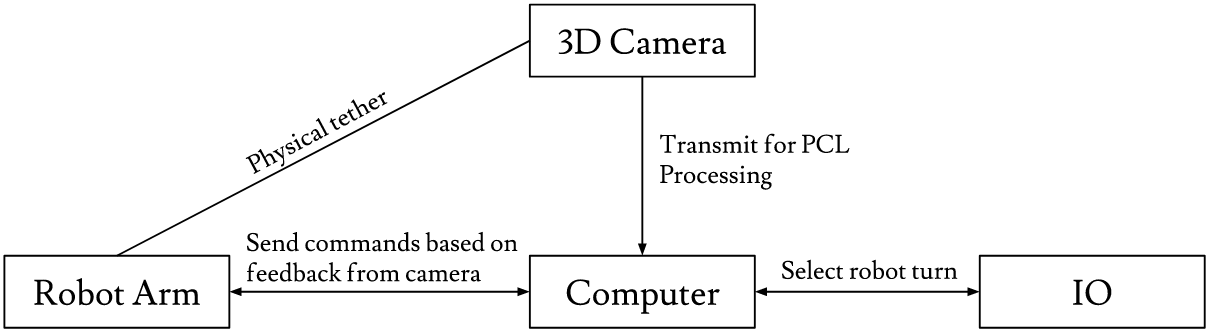
\includegraphics[width=0.8\linewidth]{images/sys_overview.png}
\caption{System Overview.}
\end{figure}

As shown in the diagram, our system consists of a UR5 robotic arm (with gripper), which is connected to a computer that handles the main processing, a 3D Camera to scan the playing field, and an IO interface to control the state of the game. This computer is responsible for tracking the state of the robot. This state can be defined as waiting for the human player to complete a turn, visually inspecting the stack for the next block pull, or performing a block pull and place based on the previously selected block. To accomplish this, the computer receives data from the camera (attached to the end effector of the robot), which is used during the scanning stage to determine the state of the Jenga stack. The state of the Jenga blocks can either be stacked or collapsed. When stacked, the goal is to find an available Jenga block, perform the pull and place, then wait for the human player to respond. In the case the Jenga stack is collapsed or collapses as a result of the robot's actions, the robot will clear a fixed playing zone of debris and begin re-stacking the blocks in place. The human opponents signals the robot via the IO interface when he or she has completed a turn.  

\begin{figure}[h!]
\centering
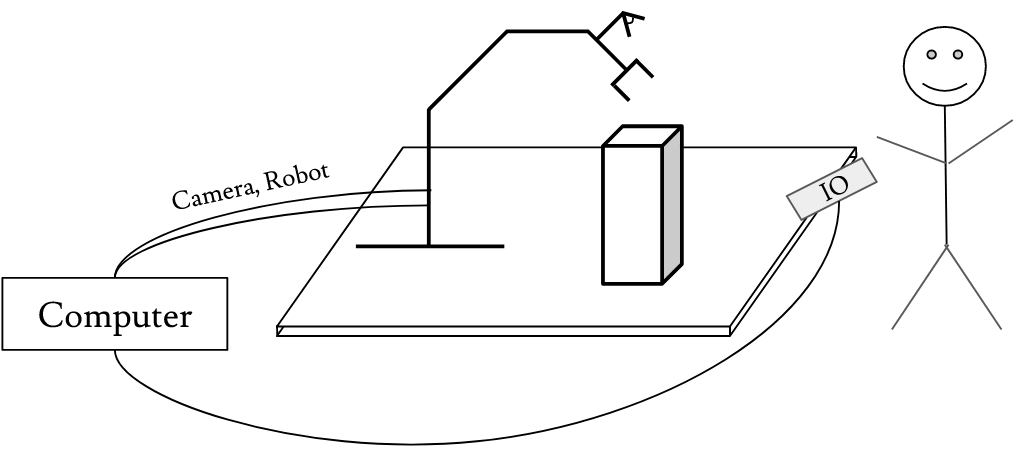
\includegraphics[width=0.78\linewidth]{images/system_setup.png}
\caption{Example Setup.}
\end{figure}